\chapter{Implementierung}\label{k_implementierung}
\section{Übersicht über die Klassenhierarchie}
Die in \cref{design_systemueberlick} vorgestellten Komponenten werden durch eine Klassenhierarchie implementiert.
Eine Gesamtübersicht der Klassenhierarchie gibt \cref{uml:class_diagram}.
Im Folgenden werden nun die einzelnen Klassen genauer betrachtet.
Im Quellcode liegen Klassen derselben Gruppe im gleichen Ordner.

\subsection{Hardware}
Die abstrakte Basisklasse dieser Gruppe ist die \identifier{Component}.
Über sie wird lediglich die entsprechende Pin-Nummer der Komponente zugeordnet.
Von \identifier{Component} erben drei Klassen: \identifier{LED}, \identifier{Sensor} sowie \identifier{Release}:

\begin{itemize}
	\item Die abstrakte Basisklasse \identifier{LED} stellt Methode zum Ein-, Aus- und Umschalten von LEDs bereit.
In den konkreten abgeleiteten Klassen (wie \identifier{GreenLED}) erfolgt dann lediglich noch die Zuordnung zum korrekten PIN.
	\item Bei \identifier{Sensor} handelt es sich ebenfalls um eine abstrakte Basisklasse, die das Abfragen von Sensoren erlaubt.
Ähnlich wie bei den LEDs wird dann in den abgeleiteten Klassen \identifier{PhotoSensor}, \identifier{HallSensor} und \identifier{Trigger} nur noch die PIN-Nummer korrekt gesetzt.
	\item Die konkrete Klasse \identifier{Release} kapselt die konkrete Ansteuerung des Servomotors, und stellt diese über die Methoden \identifier{open()} und \identifier{close()} zur Verfügung.
\end{itemize}

\begin{figure}[htb!] \centering
	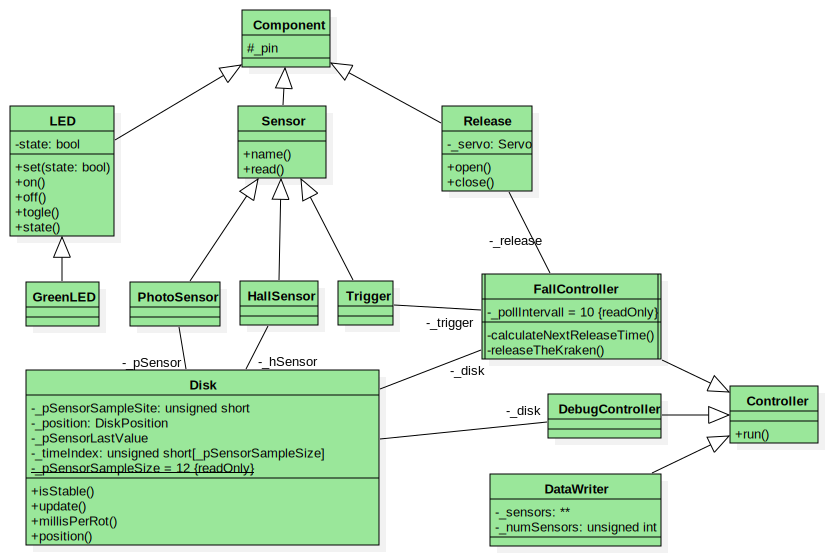
\includegraphics[width=\textwidth]{UML/class_diagram.pdf}
	\caption{Klassendiagramm der Implementierung}
	\label{uml:class_diagram}
\end{figure}

\subsection{Model}
In dieser Gruppe befindet sich nur die Klasse \identifier{Disk}, die folgende öffentliche Methoden bereitstellt:
\begin{itemize}
	\item \identifier{update()} realisiert die Aktualisierung des inneren Zustandes, also der Sensormesswerte (siehe \cref{design_aktualisierung})
	\item \identifier{position()} gibt die aktuellste Positionsmessung zurück (siehe \cref{design_pos})
	\item \identifier{millisPerRot()} gibt die aktuellste Schätzung für die Umlaufdauer zurück.
	Die Berechnung ist in \cref{design_geschwindigkeit} beschrieben.
	\item \identifier{isStable()} prüft die Sensorwerte mit den Tests aus \cref{design_stabilitaet} auf Plausibilität.
	\item \identifier{invalidate()} invalidiert 5 Sensorwerte.
	Diese Methode ist muss jeweils nach dem aktivieren des Servomotors (\identifier{open()} beziehungsweise \identifier{close()} des Release) aufgerufen werden.
\end{itemize}

Konzeptuell gilt für diese Klasse noch, dass beim (häufigen) Aktualisieren der Messwerte (via \identifier{update()}) nur die minimal nötigen Berechnungen durchgeführt werden.
Die aufwendigeren Berechnungen, vor allem für die Umlaufzeit, werden nur beim (selteneren) Aufruf der Methode \identifier{millisPerRot()} ausgeführt.

\subsection{Controller}
Controller-Klassen müssen gemäß ihrer abstrakten Basisklasse \identifier{Controller} lediglich eine \identifier{run()}-Methode implementieren.
In dieser Methode ist die Hauptschleife des Programms implementiert, so dass sie eine ähnlichen Zweck erfüllt wie die \identifier{loop()}-Funktion von Arduino.
Im Sinne eines objektorientierten Designs wurde aber von der Verwendung der \identifier{loop()}-Funktion abgesehen.

Der Kontrollfluss soll dabei den Controller nur für kurze Abfragen und Anweisungen verlassen, Methoden anderer Klassen also nicht blockieren.
Insbesondere soll es keine Delay-Anweisungen außerhalb des Controllers geben.
Durch diese Einschränkung ist sichergestellt, das regelmäßige Sensorabfragen vom Controller aus möglich sind.

Die Funktion des für die Aufgabenstellung relevanten Controllers (\identifier{FallController}) wird im folgenden Abschnitt genauer erläutert.

\section{Laufzeitverhalten}
\subsection{Objekterzeugung und Speicherverwaltung}
Prinzipiell muss bei der Programmierung in C++ die Speicherverwaltung von Objekten, die auf dem Heap alloziert werden, manuell erfolgen.
Im vorliegenden System müssen allerdings nach der Initialisierung keine Objekte auf dem Heap mehr angelegt werden.
Zugleich bleiben die initial erzeugten Objekte über die gesamte Laufzeit des Programms in Verwendung, sodass hier auf Delete-Anweisungen verzichtet werden kann.

\subsection{Kontrollfluss}
Der Kontrollfluss ist in den UML-Diagrammen in \cref{uml:statechart} und in \cref{uml:activity_diagram} dargestellt.
Zunächst ist zu beachten, das -- wie bereits in \cref{k_design} erläutert -- sämtliche Wartevorgänge alle 10 Millisekunden durch Sensorabfragen unterbrochen werden.

Zu diesen Sensorabfragen gehören einerseits die Hall- und Photo-Sensoren, anderseits aber auch der Trigger.
Letzterer wird in einer Zählvariable gehalten, und inkrementiert, sobald eine 0-1-Flanke detektiert wurde.
Zusätzlich wurde der Trigger mit einem \enquote{Cooldown}-Intervall versehen, um eine Entprellung zu realisieren.

\begin{figure}[htb!] \centering
	\begin{subfigure}[b]{0.4\textwidth}
		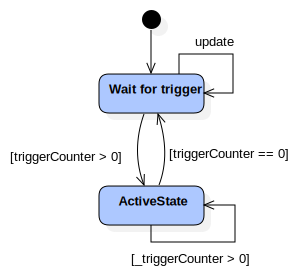
\includegraphics[width=\textwidth]{UML/fallcontroller_simple_loop_statechart.pdf}
		\caption{Einfache Darstellung}
		\label{uml:statechart_simleloop}
	\end{subfigure}\hspace{1cm}
	\begin{subfigure}[b]{0.4\textwidth}
 		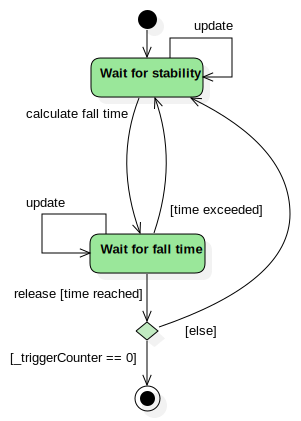
\includegraphics[width=\textwidth]{UML/fallcontroller_active_state_statechart.pdf}
		\caption{Genauere Beschreibung des ActiveStates aus \ref{uml:statechart_simleloop}}
		\label{uml:statechart_activeState}
	\end{subfigure}
	\caption{Beschreibung der Hauptschleife als Zustandsübergangsdiagramm}
	\label{uml:statechart}
\end{figure}

Bei jedem Durchlauf der Hauptschleife werden die Sensorwerte aktualisiert, und anschließend 10 Millisekunden abgewartet.
Sobald die Zählvariable größer als 0 ist, geht das System in den aktiven Zustand über.
In diesem wird zunächst die Stabilität der Sensorwerte überprüft.
Sobald die Werte stabil sind, und das passende Zeitfenster erreicht wurde, wird das Release betätigt.

Zuletzt wird dann noch die Zählvariable dekrementiert.
Auch während des Wartens auf stabilen Zustand der Scheibe sowie auf das Zeitfenster erfolgt natürlich eine kontinuierliche Abfrage der Sensoren und des Triggers alle 10 Millisekunden.

\begin{figure}[htb!] \centering
	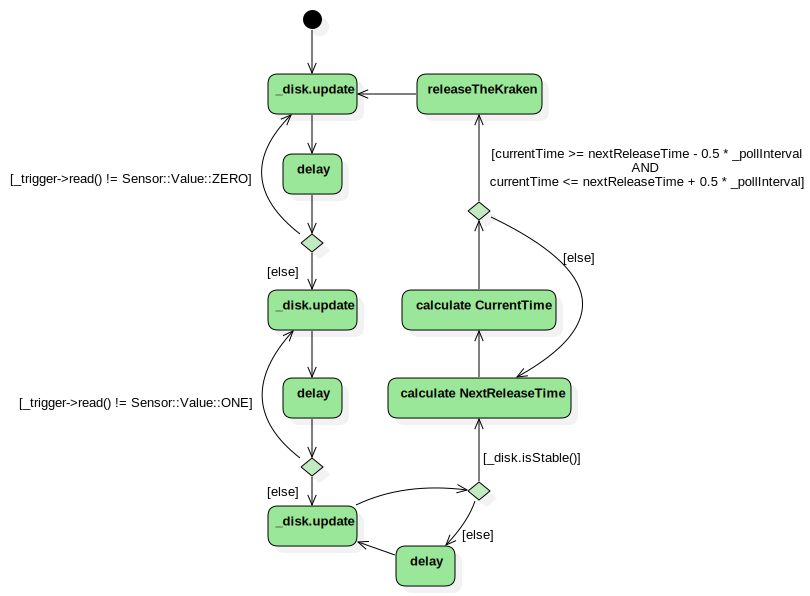
\includegraphics[width=\textwidth]{UML/fallcontroller_loop_activity_diagram.pdf}
	\caption{Genauere Beschreibung der Hauptschleife als Aktivitätsdiagramm}
	\label{uml:activity_diagram}
\end{figure}

Prinzipiell wäre es auch möglich gewesen, anstatt regelmäßiger Abfragen Interrupts zu verwenden.
Jedoch wurde der bereits in \cref{k_design} angesprochene Fehler in Bezug auf ungültige Sensorwerte zunächst auf einen Fehler im Interrupt-Handling des Arduino zurückgeführt, woraufhin von einer Verwendung von Interrupts abgesehen wurde.
Durch ein entsprechend kurzes Abfrageintervall von 10 Millisekunden in Verbindung mit nichtblockierenden Methodenaufrufen kann dennoch ein \enquote{Verpassen} von Signalen vermieden werden.

\section{Validierung}
Zum Test der Funktion des Programms wurde eine Messreihe mit 41 Versuchen durchgeführt.
Von diesen waren 34 Treffer, was einer Rate von 83 \% entspricht.
Zusätzlich wurde für jeden Versuch die Scheibengeschwindigkeit aufgezeichnet.
Die Verteilung der Messwerte zeigt \cref{img:auswertungsplot}.

\begin{figure}[htb!] \centering
	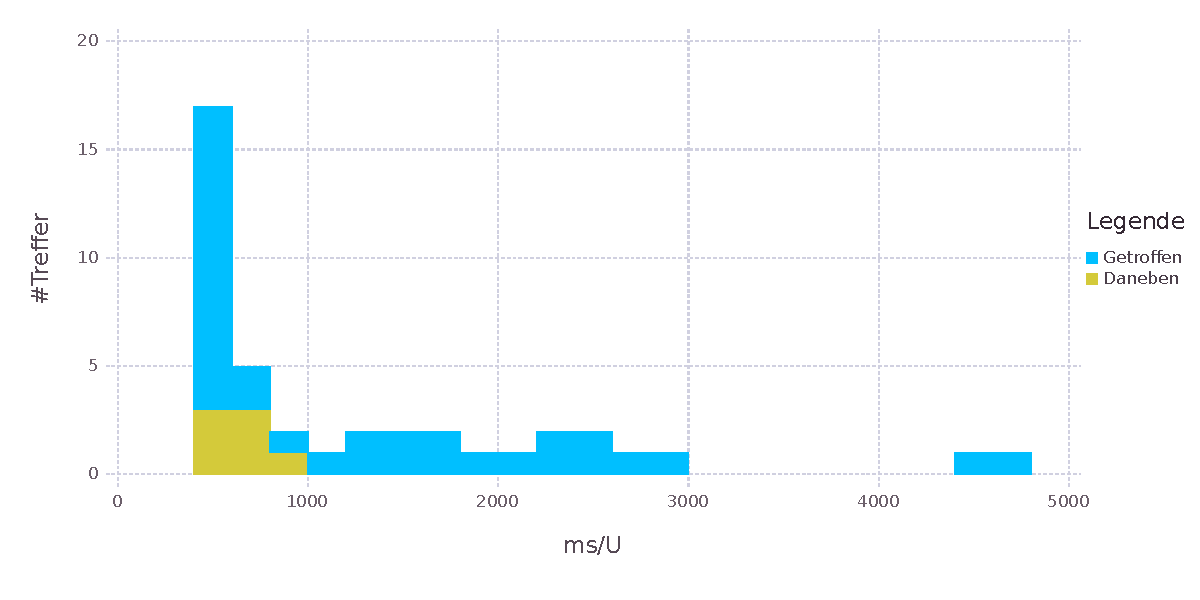
\includegraphics[width=\textwidth]{images/auswertung.pdf}
	\caption{Auswertung der Trefferzahlen über der Drehgeschwindigkeit (Intervallgröße: 200\,ms)}
	\label{img:auswertungsplot}
\end{figure}

Die fehlerhaften Versuche liegen alle im Bereich von Umlaufdauern unter einer Sekunde.
Vermutlich liegt die Ursache darin, dass die Toleranzbereiche für Fehler bei höheren Geschwindigkeiten kleiner sind.
Zudem wurde die Approximation der Umlaufdauern (beschrieben in \cref{subs:dreh_approx}) für den anderen Versuchsaufbau erzeugt.
Bedingt durch einen fehlerhaften Photosensor musste der Aufbau dann aber kurzfristig gewechselt werden.

\section{Sonstiges}
Für die gemeinsame Softwareentwicklung wurde Git als Versionskontrollsystem verwendet.\footnote{Repository: \url{https://github.com/mp1409/kislab}}
Um einen stets kompilierbaren Zustand des Codes zu erreichen, kam der Continious-Integration-Dienst von Travis zum Einsatz.\footnote{Travis: \url{https://travis-ci.org/mp1409/kislab/branches}}
Die Quelltextdokumentation wurde mit Doxygen generiert.
